% fig8-call-chain.tex — Figure 8: Review call chain (DEV-GOV-03)
%
% One `sego sidecar review` invocation, function by function, with the point at
% which each artifact identity is decided. The chain is drawn as a single column
% because it is single-threaded and ordered: everything below a step happens only
% if the step above it succeeded.
%
% Anchored in the code: names are the real callables, and the file coordinates are
% the ones the development issue list uses.
\documentclass[tikz,border=10pt]{standalone}
\usetikzlibrary{arrows.meta,positioning,fit,backgrounds,calc}

\begin{document}
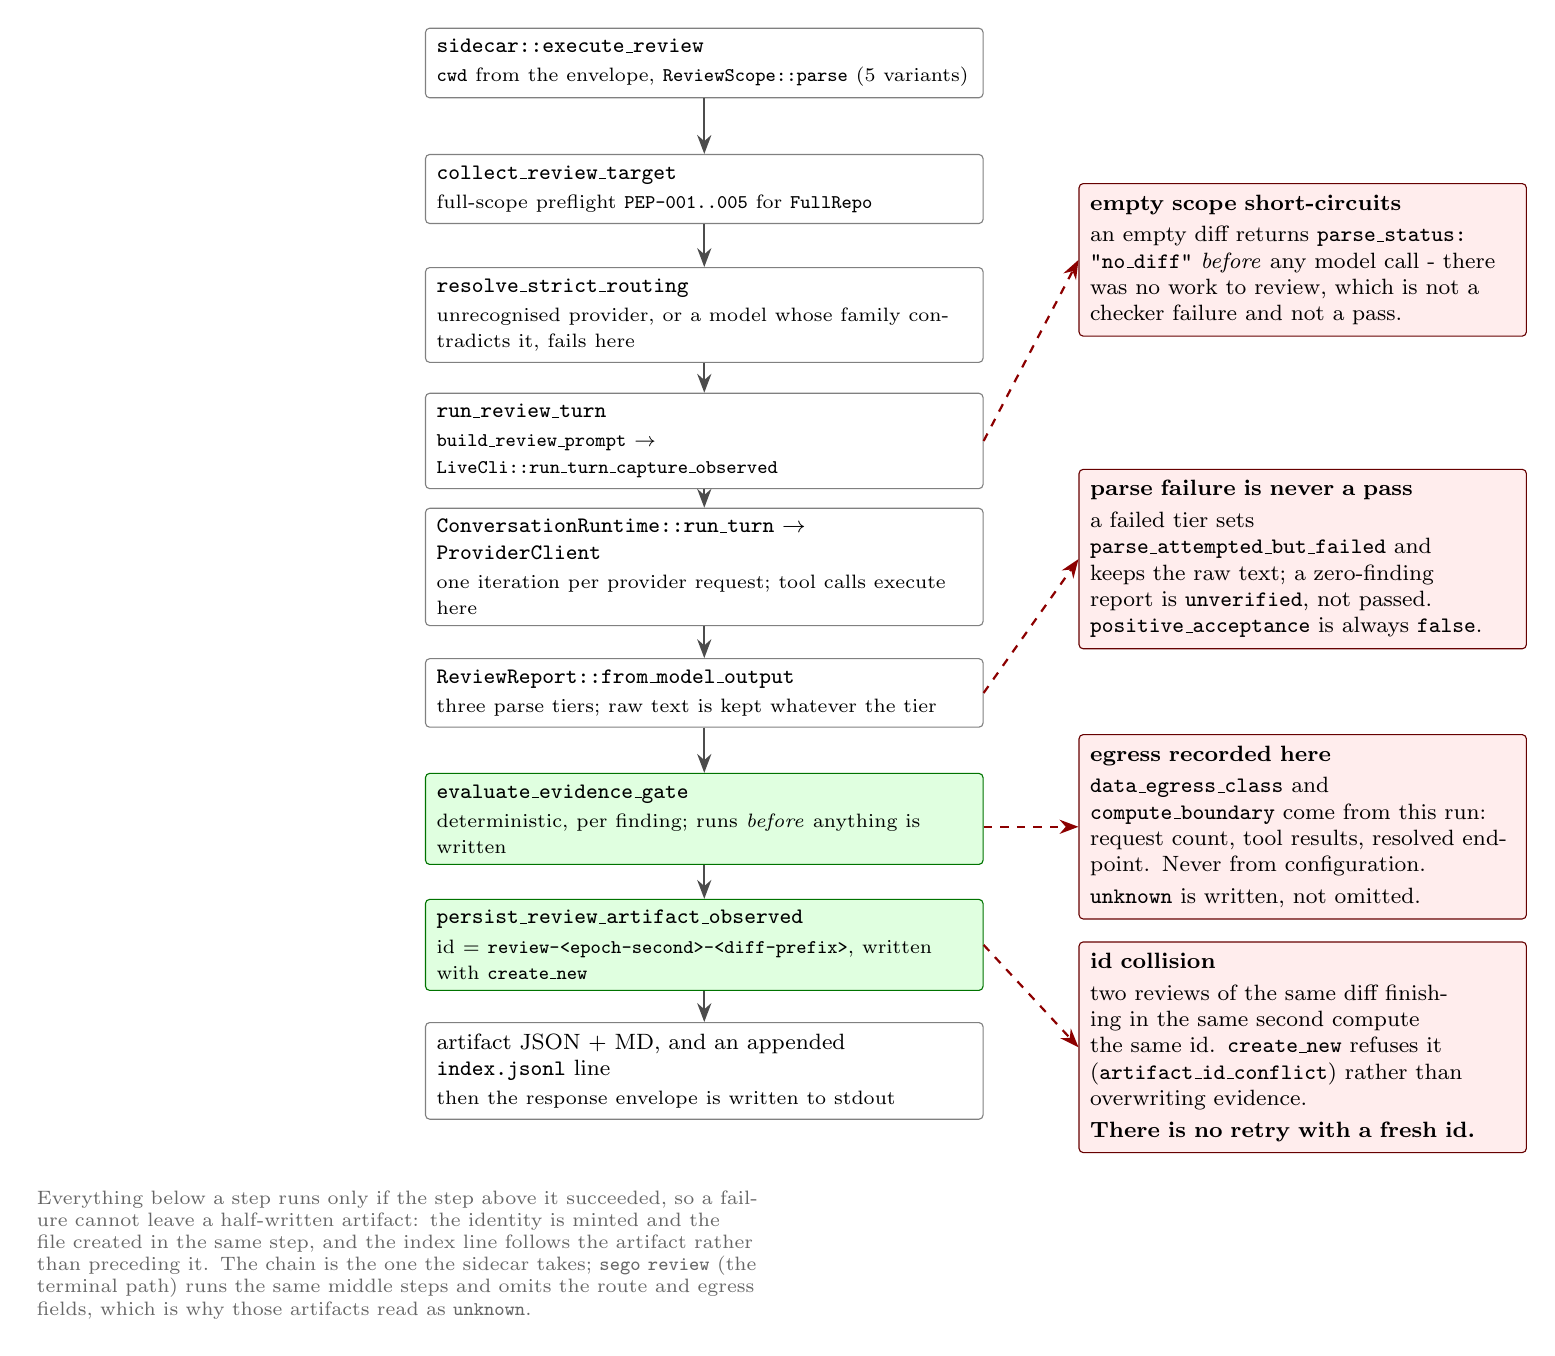
\begin{tikzpicture}[
  x=1cm, y=1cm,
  font=\small,
  bx/.style={draw, rounded corners=1.5pt, fill=white, draw=black!50,
               font=\footnotesize, align=left, inner sep=4pt, text width=68mm},
  gatebox/.style={bx, fill=green!12, draw=green!45!black},
  callout/.style={bx, fill=red!7, draw=red!40!black, text width=54mm},
  arr/.style={-{Stealth[length=2.4mm]}, thick, draw=black!70},
  farr/.style={-{Stealth[length=2.4mm]}, thick, draw=red!55!black, dashed},
  lab/.style={font=\scriptsize, text=black!65, inner sep=2pt, fill=white},
  grp/.style={draw=black!25, dashed, rounded corners=3pt, inner sep=7pt}
]

\node[bx] (s1) at (0, 8.6)
  {\texttt{sidecar::execute\_review}\\[1pt]
   \scriptsize \texttt{cwd} from the envelope, \texttt{ReviewScope::parse} (5 variants)};
\node[bx] (s2) at (0, 7.0)
  {\texttt{collect\_review\_target}\\[1pt]
   \scriptsize full-scope preflight \texttt{PEP-001..005} for \texttt{FullRepo}};
\node[bx] (s3) at (0, 5.4)
  {\texttt{resolve\_strict\_routing}\\[1pt]
   \scriptsize unrecognised provider, or a model whose family contradicts it, fails here};
\node[bx] (s4) at (0, 3.8)
  {\texttt{run\_review\_turn}\\[1pt]
   \scriptsize \texttt{build\_review\_prompt} $\rightarrow$ \texttt{LiveCli::run\_turn\_capture\_observed}};
\node[bx] (s5) at (0, 2.2)
  {\texttt{ConversationRuntime::run\_turn} $\rightarrow$ \texttt{ProviderClient}\\[1pt]
   \scriptsize one iteration per provider request; tool calls execute here};
\node[bx] (s6) at (0, 0.6)
  {\texttt{ReviewReport::from\_model\_output}\\[1pt]
   \scriptsize three parse tiers; raw text is kept whatever the tier};
\node[gatebox] (s7) at (0, -1.0)
  {\texttt{evaluate\_evidence\_gate}\\[1pt]
   \scriptsize deterministic, per finding; runs \emph{before} anything is written};
\node[gatebox] (s8) at (0, -2.6)
  {\texttt{persist\_review\_artifact\_observed}\\[1pt]
   \scriptsize id = \texttt{review-<epoch-second>-<diff-prefix>}, written with \texttt{create\_new}};
\node[bx] (s9) at (0, -4.2)
  {artifact JSON + MD, and an appended \texttt{index.jsonl} line\\[1pt]
   \scriptsize then the response envelope is written to stdout};

\draw[arr] (s1) -- (s2);
\draw[arr] (s2) -- (s3);
\draw[arr] (s3) -- (s4);
\draw[arr] (s4) -- (s5);
\draw[arr] (s5) -- (s6);
\draw[arr] (s6) -- (s7);
\draw[arr] (s7) -- (s8);
\draw[arr] (s8) -- (s9);

% ---------------- where the identity is decided ----------------
\node[callout] (idc) at (7.6, -3.9)
  {\textbf{id collision}\\[2pt] two reviews of the same diff finishing in the same
   second compute the same id. \texttt{create\_new} refuses it (\texttt{artifact\_id\_conflict})
   rather than overwriting evidence.\\[2pt] \textbf{There is no retry with a fresh id.}};
\draw[farr] (s8.east) -- (idc.west);

\node[callout] (egr) at (7.6, -1.1)
  {\textbf{egress recorded here}\\[2pt] \texttt{data\_egress\_class} and
   \texttt{compute\_boundary} come from this run: request count, tool results, resolved
   endpoint. Never from configuration.\\[2pt] \texttt{unknown} is written, not omitted.};
\draw[farr] (s8.east |- egr.west) -- (egr.west);

\node[callout] (pf) at (7.6, 2.3)
  {\textbf{parse failure is never a pass}\\[2pt] a failed tier sets
   \texttt{parse\_attempted\_but\_failed} and keeps the raw text; a zero-finding report is
   \texttt{unverified}, not passed. \texttt{positive\_acceptance} is always \texttt{false}.};
\draw[farr] (s6.east) -- (pf.west);

\node[callout] (empty) at (7.6, 6.1)
  {\textbf{empty scope short-circuits}\\[2pt] an empty diff returns
   \texttt{parse\_status: "no\_diff"} \emph{before} any model call - there was no work to
   review, which is not a checker failure and not a pass.};
\draw[farr] (s4.east) -- (empty.west);

\node[font=\scriptsize, text=black!60, text width=92mm, align=left, anchor=north west] at (-8.6, -5.6)
  {Everything below a step runs only if the step above it succeeded, so a failure cannot leave a half-written artifact: the
   identity is minted and the file created in the same step, and the index line follows the artifact rather than preceding it.
   The chain is the one the sidecar takes; \texttt{sego review} (the terminal path) runs the same middle steps and omits the
   route and egress fields, which is why those artifacts read as \texttt{unknown}.};

\end{tikzpicture}
\end{document}
